\documentclass[11pt]{article}

\usepackage[margin=1in]{geometry}
\usepackage{amsmath,amssymb}
\usepackage{booktabs}
\usepackage{graphicx}
\usepackage{float}
\usepackage{placeins}
\usepackage{microtype}
\usepackage[font=small,labelfont=bf]{caption}
\usepackage[numbers,sort&compress]{natbib}
\usepackage[hidelinks]{hyperref}

\graphicspath{{../figures/preprint/}}
\setlength{\parindent}{0pt}
\setlength{\parskip}{0.65em}
\emergencystretch=2em
\raggedbottom

\title{Readout-compatible CA1 plasticity supports cue-dependent reconfiguration and degraded-cue recall in a minimal hippocampal model}
\author{Author Name}
\date{}

\begin{document}
\maketitle

\begin{abstract}
Rapid episodic memory requires not only selecting stored content, but expressing
that content in a form that downstream circuits can interpret. We examine this
constraint in a minimal hippocampal model in which entorhinal cortex (EC)
generates a CA3-like retrieval key and an instructed CA1 state, plastic
CA3--CA1 weights associate the key with that state, and a fixed pretrained
CA1--EC decoder reconstructs the input. Pretraining establishes a
representational basis before rapid associative learning. Across 20 paired
initializations, a fixed permutation of the instructed CA1 coordinates impaired
one-shot reconstruction under both an instructive-driven rule (mean
output--target cosine, 0.804 aligned versus 0.125 permuted) and a bounded
error-driven rule (0.514 versus 0.066). Applying the corresponding permutation
to the decoder restored performance, demonstrating that preserved information
can become unreadable to an unchanged output pathway. On a cue-guided circular
track, exchanging cue identities caused abrupt, reproducible changes in CA1
tuning relative to a matched no-swap control. Event-aligned and population-map
analyses revealed a transient update at exchange boundaries and alternating
representational blocks tied to cue assignment. Both rules generated
continuous mixtures of spatially stable and cue-modulated responses, while differing
quantitatively in one-shot reconstruction, tuning stability, and position
decodability. During frozen recall, selective degradation of lateral or medial
EC inputs preferentially impaired cue or position readout, respectively, while
the complementary cue readout was preserved under medial EC degradation. A
dense common-key control failed to distinguish cue or position states. These
simulations support a limited proposal: CA3-like keys can select associative
content, while rapid CA1 plasticity expresses that content within a structured
basis that remains legible to an established readout. The model demonstrates
degraded-cue robustness, not recurrent CA3 pattern completion or long-term
stability.
\end{abstract}

\section{Introduction}

The hippocampal formation is commonly modeled as a system capable of rapidly encoding conjunctive representations of individual episodes and retrieving them from partial cues.
In hippocampal-indexing and complementary-learning-systems theories, this role is formalized as rapid storage of episodic representations alongside slower cortical learning \citep{teyler1986,mcclelland1995}.
An effective memory system must therefore distinguish related episodes, select or reconstruct an appropriate stored state, and express the resulting representation in a form usable by downstream circuits.
The first requirement is central to theories of pattern separation, whereas the second is closely related to pattern completion and attractor-based retrieval.
Here we focus on the third: the representational coordinates in which retrieved content is expressed.
This motivates a view of CA1 not merely as a relay or container of individual memories, but as an adaptive interface that organizes successive experiences within a structured neural space.

The anatomy of the hippocampal formation suggests a distribution of computational roles across its subfields.
Entorhinal cortex (EC) provides major cortical input to the hippocampus.
Medial EC (MEC) is often associated with path integration, spatial metrics, and environmental geometry, whereas lateral EC (LEC) is more strongly associated with local sensory, object, and event-related information.
However, both regions contain mixtures of spatial and nonspatial signals, and their relative contributions depend on behavioral context and task demands \citep{hargreaves2005,henriksen2010,deshmukh2011}.
The canonical trisynaptic circuit conveys entorhinal layer II input through dentate gyrus and CA3 to CA1, whereas entorhinal layer III provides a direct temporoammonic projection to CA1.
Autoassociative models assign recurrent CA3 circuitry a central role in content-addressable retrieval \citep{marr1971}.
Consistent with this view, selective disruption of CA3 NMDA-receptor function impairs recall from partial cues, and CA3 and CA1 ensembles can exhibit regionally distinct responses to environmental change \citep{nakazawa2002,leutgeb2004}.
These accounts provide mechanisms by which a stored activity pattern could be selected or completed, but they do not by themselves specify the representational coordinates in which the resulting activity should be expressed at hippocampal output.

CA1 representations can form and reorganize rapidly.
Behavioral-timescale synaptic plasticity (BTSP) can create a place field after a single dendritic plateau event and can bidirectionally reshape an existing field according to its relation to the instructive event \citep{bittner2017,milstein2021}.
EC layer 3 activity has been implicated as an instructive or teaching-related signal for learning-dependent changes in CA1 population activity \citep{grienberger2022}.
Recent experiments and models further connect BTSP-like dynamics to trial-by-trial field shifts and the stabilization of task-relevant spatial codes \citep{madar2025,vaidya2025}.
BTSP is therefore potentially relevant not only to the formation of isolated place fields but also to the rapid updating of spatial representations when cues or task contingencies change.
Computational work additionally shows that BTSP-like rules can support rapid content-addressable storage \citep{wu2025}.
The present study abstracts this motif as an EC-related instructive signal that modifies CA3--CA1 synaptic weights; it does not model the temporal eligibility trace, dendritic plateau potential, or molecular mechanisms of biological BTSP.

CA1 activity is also context sensitive.
Changes in environmental or cue configuration can alter firing rates, field locations, and the active ensemble, producing phenomena commonly described as rate remapping and global remapping \citep{muller1987,leutgeb2005}.
Direct entorhinal input provides a route by which spatial and nonspatial variables can jointly shape these changes.
In the model below, separate MEC-like and LEC-like input partitions provide a controlled way to manipulate those variables.
This is a modeling abstraction used to test pathway-selective perturbations, not a claim that biological MEC and LEC carry pure or independent information channels.

Our central proposal adds a representational constraint to this circuit motif.
If rapid plasticity writes a CA1 pattern while the downstream readout remains fixed, the pattern may retain information about an episode yet become functionally unusable if it falls outside the activity subspace or coordinate system to which the readout is tuned.
Related constraints have been demonstrated outside the hippocampus.
In brain--computer-interface experiments, motor-cortical perturbations that remained within a pre-existing neural manifold were learned more readily than perturbations requiring activity outside that manifold \citep{sadtler2014}; short-term adaptation could also occur by reassociating an established cortical activity repertoire with new behavioral outputs \citep{golub2018}.
Stable population-level dynamics can preserve behavioral representations despite substantial changes in the participation of individual neurons \citep{gallego2020}.
These findings motivate the possibility that established downstream mappings constrain which newly learned population states can be used effectively.
We use the narrower term \emph{readout compatibility} for the requirement that a newly instructed CA1 state remain within the subset of population activity space that an established output mapping can interpret correctly.
Readout compatibility is therefore a functional criterion, whereas manifold preservation is one possible geometric mechanism by which compatibility could be maintained.

To instantiate prior structure, an EC--CA1--EC autoencoder is pretrained before new associations are stored.
This is a computational device, not a claim that CA1 is biologically optimized by backpropagation in a separate phase.
Biologically, the pretrained mapping is intended as an abstraction of structure accumulated through development, prior experience, and relatively stable connectivity between entorhinal and hippocampal circuits \citep{mcclelland1995,chandra2025,wen2024}.
In deep learning, pretraining can play an analogous engineering role by establishing reusable features before rapid adaptation, although the mechanisms, objectives, and substrates differ \citep{yosinski2014}.
Freezing the decoder after pretraining turns compatibility into an explicit assay: a new CA1 state must remain legible to the established readout rather than being rescued by encoder--decoder co-adaptation.
Such a relation could, in principle, support stable decoding across successive experiences, but long-term stability is not tested here.

We study this idea in a deliberately minimal model.
EC input is transformed into two representations: a discriminable CA3-like retrieval key and a pretrained instructed CA1 target state.
Plastic CA3--CA1 synapses associate the key with that target state, and a frozen CA1--EC decoder reconstructs the recalled representation.
We compare an instructive-driven rule with a bounded error-driven rule that corrects the discrepancy between instructed and recalled CA1 activity.
The simulations ask whether accurate reconstruction depends on coordinate compatibility, whether cue-sequence changes induce reproducible CA1 reconfiguration, and how the two update rules differ under matched conditions and near separately selected operating points.
We further test how recall changes when MEC-like or LEC-like EC input is selectively degraded, and how exact pattern-recall accuracy changes as more ordered cue pairs are stored.
The resulting claims are constructive and conditional: the model proposes a representational principle and exposes its consequences, but does not establish that biological CA3 or CA1 implements the exact architecture, pretraining procedure, or synaptic rules used here.

\section{Results}

\subsection{A minimal retrieval-key and instructed-CA1 architecture}

The model contains four functional components (Fig.~\ref{fig:model}A).
Entorhinal input, denoted $x_{\mathrm{EC}}$, projects through a fixed sparse
map to a CA3-like population that provides a retrieval key. A separately
pretrained EC--CA1 encoder transforms the same input into an instructed CA1
state (IS). Plastic CA3--CA1 weights associate the retrieval key with the IS,
whereas the corresponding pretrained CA1--EC decoder remains fixed. During
recall, the EC input regenerates a key, the learned association reconstructs a
CA1 state, and the decoder maps that state back to EC output. This architecture
separates the selection of associative content from its expression in a
pre-existing output basis.

We first evaluated two plasticity rules under matched inputs and a shared
reference parameter configuration
(Fig.~\ref{fig:model}B). The instructive-driven rule writes an outer-product
association gated by the IS without considering the current recalled state.
The bounded error-driven rule instead potentiates CA3--CA1 synapses for underexpressed
CA1 components and depresses them for overexpressed components. Repeated
presentations therefore rewrite the instructed association under the instructive-driven
rule but correct a residual under the error-driven rule. Both are abstract
models of rapid instructed plasticity; neither implements the temporal
eligibility trace or dendritic plateau dynamics of biological BTSP.

Track inputs combined a MEC-like spatial component with a LEC-like cue
component (Fig.~\ref{fig:model}D). Two cue identities occurred at fixed
positions and could exchange locations across blocks. For degradation tests,
the model first stored intact laps; plasticity was then frozen while a fixed
fraction of either the MEC-like or LEC-like input units was set to zero
(Fig.~\ref{fig:model}E).

\begin{figure}[!htbp]
    \centering
    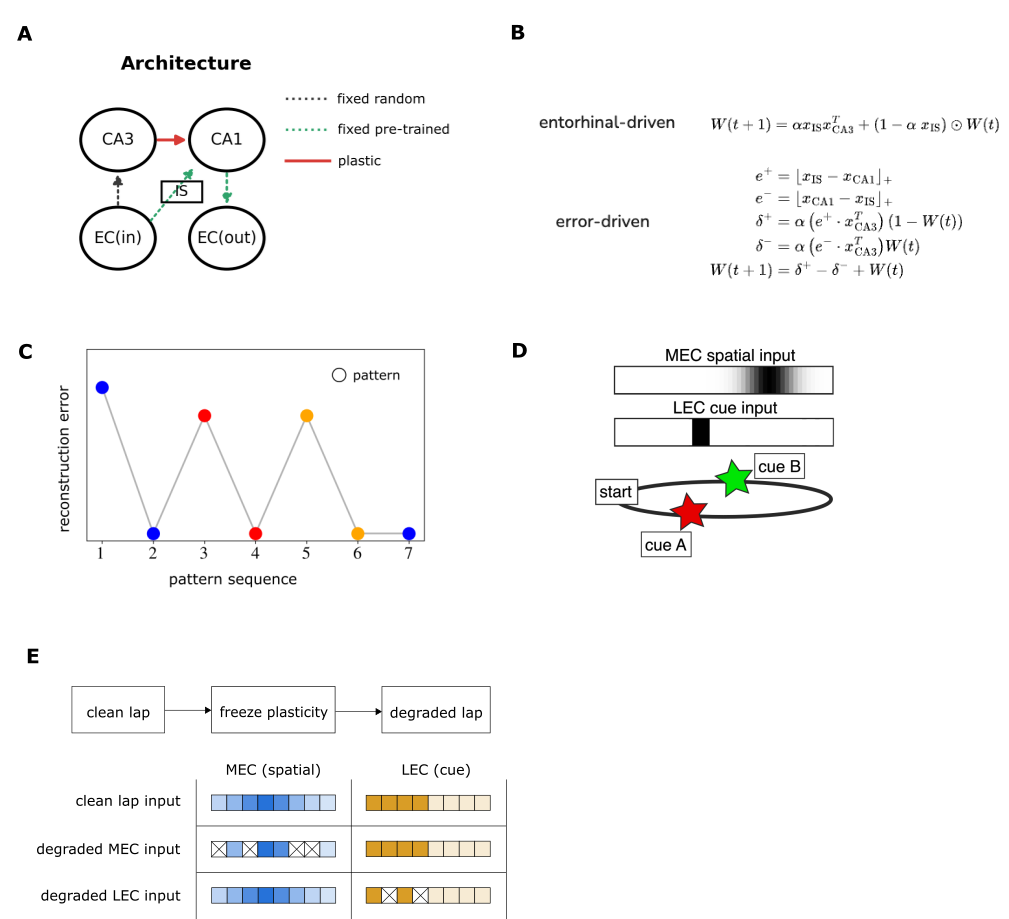
\includegraphics[width=\textwidth]{figure_1.png}
    \caption{\textbf{Model architecture and simulation protocol.}
    \textbf{(A)} EC input produces a fixed sparse CA3-like retrieval key
    $x_{\mathrm{CA3}}$ and, through a pretrained encoder, an instructed CA1
    state $x_{\mathrm{IS}}$. Plastic
    CA3--CA1 weights store their association; a fixed pretrained CA1--EC
    decoder reads out recall. \textbf{(B)} Instructive-driven and bounded
    error-driven update rules.
    \textbf{(C)} Conceptual reconstruction-error trajectories over first and
    repeated presentations; colors denote pattern identity. This panel is a
    schematic rather than a measured result. \textbf{(D)} Circular-track input
    composed of MEC-like spatial activity and LEC-like cue activity.
    \textbf{(E)} Selective degradation protocol. Intact laps are stored before
    plasticity is frozen; a fraction of MEC-like or LEC-like units is then
    zeroed using a mask held fixed within a probe lap and resampled across
    probes.}
    \label{fig:model}
\end{figure}

\subsection{Readout compatibility constrains rapid associative storage}

We first isolated the relationship between an instructed CA1 code and its fixed
output decoder (Fig.~\ref{fig:compatibility}A). Twenty independently
initialized autoencoders were pretrained on structured MEC+LEC patterns and
then frozen. Pattern order was shuffled, so this assay retained the marginal
spatial--cue structure without presenting a traversed track sequence.
For each initialization, 28 held-out patterns were stored once under five
paired conditions. In the aligned condition, the IS remained in the
coordinates learned by the decoder. In the fixed-permutation condition, the
same non-identity permutation was applied to every IS while the decoder was
left unchanged. In the matched-decoder condition, the corresponding decoder
columns were permuted together with the IS. Random-content and no-plasticity
conditions controlled for storing an incorrect association and for leaving the
memory unwritten, respectively.

Under the instructive-driven rule, aligned instructions produced a mean output--target
cosine of 0.880 (95\% confidence interval [CI], 0.870--0.891), whereas a fixed
coordinate permutation reduced it to 0.247 (0.207--0.286). The paired
aligned-minus-permuted difference was 0.634 (0.592--0.676). The same coordinate
dependence appeared under the error-driven rule: aligned and permuted means
were 0.872 (0.858--0.887) and 0.178 (0.147--0.209), respectively, giving a
paired difference of 0.694 (0.658--0.731). Permuting the decoder together with
the IS restored the aligned mean exactly for each rule. Random-content recall
remained lower (0.355 for the instructive-driven rule and 0.315 for the
error-driven rule), as did the shared
no-plasticity control (0.114). The matched-decoder restoration is an algebraic
coordinate control: the permutation preserves the IS values but changes their
meaning to the unchanged decoder. Reconstruction therefore depends on
compatibility between the instructed CA1 coordinates and the fixed output
basis, not on information content alone. Under this reference configuration,
the two rules reached similar aligned one-shot recall despite using different
update signals: the instructive-driven rule performs a full instructed write,
whereas the error-driven rule makes a bounded residual correction.

\subsection{Cue exchanges induce reproducible CA1 reconfiguration}

We next exposed the model to 40 track laps in which two cue identities exchanged
positions every 10 laps (Fig.~\ref{fig:compatibility}B). A paired no-swap
control used the same root seeds, pretrained encoder and decoder, MEC-like
trajectories, lap count, plasticity parameters, and exact EC--CA3 projection,
but retained the initial cue assignment throughout.
After every training lap, plasticity was paused and the model was probed in the
context scheduled for that lap.

For the instructive-driven rule, mean unit-wise tuning similarity between consecutive probes
fell to 0.365 at cue exchanges (95\% CI, 0.348--0.382), compared with 0.845 at
the same lap boundaries in the no-swap control (0.832--0.857). The paired
swap-minus-control difference was $-0.479$ ($-0.498$ to $-0.461$). Under the
error-driven rule, exchange-boundary similarity was 0.451 (0.436--0.466),
compared with 0.827 in the matched control (0.817--0.838), for a paired
difference of $-0.376$ ($-0.396$ to $-0.356$). At non-exchange transitions in
the alternating schedule, similarity remained high for both the instructive-driven
rule (0.833, 0.823--0.843) and the error-driven rule (0.821, 0.814--0.828).
The abrupt tuning changes were
therefore associated with the altered cue sequence rather than with continued
learning alone.

We next aligned the three exchange events to their first post-exchange lap
(Fig.~\ref{fig:compatibility}E). Under the instructive-driven rule,
consecutive-lap similarity at the exchange was 0.375 (95\% CI,
0.351--0.398), versus 0.851 (0.839--0.863) at matched no-swap boundaries; the
paired difference was $-0.477$ ($-0.499$ to $-0.454$). Under the error-driven
rule, the corresponding values were 0.462 (0.443--0.480) and 0.833
(0.822--0.845), with a paired difference of $-0.372$ ($-0.391$ to $-0.352$).
By the following lap, similarity recovered to 0.769 (0.756--0.783) and 0.819
(0.806--0.832), respectively. Thus the response was concentrated at the cue
exchange rather than developing as nonspecific drift over the subsequent
block.

The lap-by-lap population representational-similarity matrix provided a
complementary view (Fig.~\ref{fig:compatibility}F). Within-block maps remained
similar, exchanges separated the sequence into distinct blocks, and
nonadjacent blocks carrying the same cue assignment resembled one another.
The model therefore alternated between cue-dependent population states rather
than accumulating a wholly novel map after every block. Retrospective
comparison with the final map of each new block further showed that the first
post-exchange representation was already closer to the eventual adapted map
than to the pre-exchange map, followed by smaller within-block changes
(Supplementary Fig.~\ref{fig:remapping-dynamics}A,B). Endpoint similarities
were broadly distributed across CA1 units, demonstrating that the population
effect was not produced by a single uniform response class
(Supplementary Fig.~\ref{fig:remapping-dynamics}C,D).

After learning, plasticity was frozen and both cue arrangements were probed.
The representative error-driven population contained spatially stable fields,
amplitude-modulated responses, and fields whose preferred position changed
with cue identity (Fig.~\ref{fig:compatibility}C). Across seeds, mean
unit-wise, mean-centered spatial stability was 0.330 (95\% CI, 0.297--0.363)
under the instructive-driven rule and 0.464 (0.441--0.486) under the
error-driven rule. Mean absolute cue modulation
was 0.132 (0.130--0.135) and 0.124 (0.120--0.128), respectively. In both rules,
the unit-level distributions were continuous rather than separated into
discrete response classes (Fig.~\ref{fig:compatibility}D), and strong cue
modulation was concentrated among units with low or negative cross-context
stability. These distributions are descriptive: units nested within a seed
were not treated as independent replicates, and the analysis is not a formal
classification of rate versus global remapping. Operationally, changing the
cue arrangement changed both the EC-derived instruction and the CA3-like key,
producing a mixture of stable and context-dependent recalled CA1 activity.

\begin{figure}[!htbp]
    \centering
    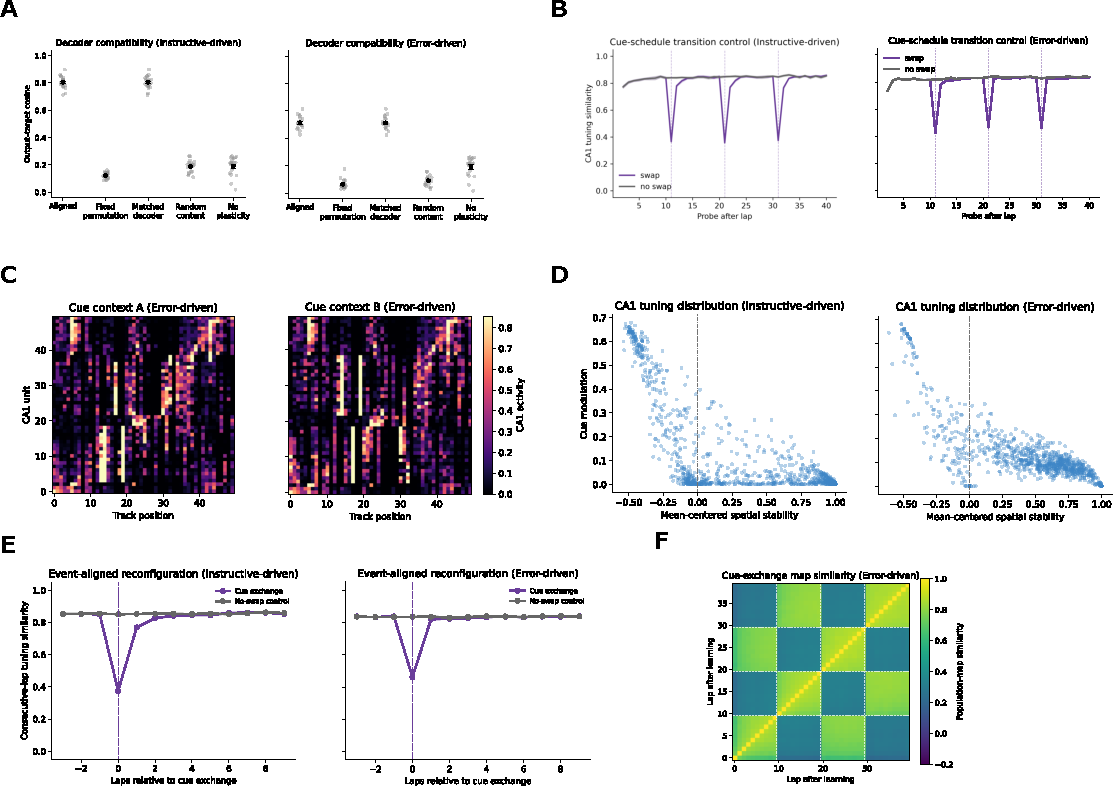
\includegraphics[width=0.98\textwidth]{figure_2.pdf}
    \caption{\textbf{Readout compatibility and cue-dependent CA1
    reconfiguration.} \textbf{(A)} Output--target cosine for shuffled MEC+LEC
    samples in aligned,
    fixed-permutation, matched-decoder, random-content, and no-plasticity
    conditions for the instructive-driven rule (left) and error-driven rule
    (right). Grey points are
    seed means across 28 stored memories; black points and error bars show mean
    $\pm$ SEM across 20 seeds. \textbf{(B)} Mean unit-wise tuning similarity
    between consecutive scheduled-context probes for the instructive-driven
    rule (left) and error-driven rule (right). Purple denotes the cue-exchange
    schedule and grey the matched
    no-swap control; vertical dashed lines mark exchanges. Curves show mean
    $\pm$ SEM across 20 paired seeds. \textbf{(C)} Recalled CA1 activity on the
    same track under cue contexts A (left) and B (right) for the representative
    error-driven seed. Units have the same order and are sorted by preferred position
    across contexts; color limits are shared. \textbf{(D)} Unit-level
    relationship between mean-centered spatial stability and cue modulation
    for the instructive-driven rule (left) and error-driven rule (right),
    pooling 50 units from each of 20 seeds
    (1,000 points per rule). The vertical line marks zero stability. Panels C
    and D illustrate heterogeneous stable and cue-dependent responses but do
    not formally classify remapping type; confidence intervals in the text use
    seed-level summaries. \textbf{(E)} Event-aligned consecutive-lap tuning
    similarity for the instructive-driven rule (left) and error-driven rule
    (right) in the cue-exchange schedule and exact-wiring no-swap control. Lap
    zero is the first post-exchange lap;
    values were averaged across three exchanges within each seed and curves
    show mean $\pm$ SEM across 20 seeds. \textbf{(F)} Error-driven
    lap-by-lap population-map similarity, averaged across 20 seeds. Before
    comparison, each unit was mean-centered over track position and the full
    position-by-unit map was vectorized. Dashed lines mark cue-exchange
    boundaries. Panels B and E used identical EC--CA3 projections in the
    exchange and no-swap schedules for each rule; panel F shows the
    error-driven exchange schedule.}
    \label{fig:compatibility}
\end{figure}

\subsection{Selective EC degradation dissociates cue and spatial readout}

We then asked whether the stored association remained usable when one EC input
modality was selectively corrupted (Fig.~\ref{fig:degradation}). Each model
stored 20 intact laps with a fixed cue arrangement. Plasticity was frozen, and
independent masks removed 0, 25, 50, 75, 90, or 100\% of eligible units. Each
fraction used 12 masks per seed and 20 paired root seeds; the numerical summary
below focuses on 90\% partial degradation. The principal control
replaced the normal sparse EC--CA3 map with a dense common map in which every
CA3-like unit received the same average EC input. This manipulation removes
item-specific key structure and is therefore a degenerate-key, not a
sparsity-matched, control.

Under LEC-like degradation, cue identity accuracy for the normal key declined
from 1.000 to 0.871 at 90\% dropout under the instructive-driven rule (95\% CI
at 90\%, 0.803--0.938) and from 1.000 to 0.829 under the error-driven
rule (0.766--0.893;
Fig.~\ref{fig:degradation}A). The corresponding 90\%-dropout changes were
$-0.129$ ($-0.197$ to $-0.062$) and $-0.171$ ($-0.234$ to $-0.107$).
MEC output--target cosine remained near its instructive-driven baseline (0.736 at
baseline and 0.723 at 90\% dropout; change $-0.013$, $-0.029$ to
$0.003$), whereas it declined from 0.904 to 0.780 under the error-driven rule
(change $-0.125$,
$-0.136$ to $-0.113$; Fig.~\ref{fig:degradation}B). Thus spatial output
remained substantially readable under LEC-like corruption, although it was not
strictly invariant under the error-driven rule.

MEC-like degradation produced the complementary loss of position information.
Nearest-position accuracy declined from 0.163 to 0.070 under the
instructive-driven rule (90\%-dropout
change $-0.093$, 95\% CI $-0.106$ to $-0.079$) and from 0.666 to 0.069 under
the error-driven rule (change $-0.597$, $-0.636$ to $-0.557$; chance $=0.02$;
Fig.~\ref{fig:degradation}C). Cue identity remained 1.000 for every seed and
degradation level under both rules (Fig.~\ref{fig:degradation}D). The low
baseline position accuracy under the instructive-driven rule is itself
informative: repeated
error-driven correction yielded a substantially more discriminable spatial
readout before degradation, whereas the instructive-driven rule did not. The two rules
should therefore not be interpreted as starting from equivalent clean spatial
performance.

The dense common-key control remained at chance for cue identity (0.5) and
position (0.02) even without degradation, and produced low spatial-output
cosine. Its failure establishes that a non-specific common key cannot support
the associations, but does not isolate sparsity from key discriminability.
Together, the normal-key results demonstrate degraded-cue robustness and
pathway-selective failure within this architecture. They do not establish
recurrent pattern completion: the CA3-like layer has no attractor dynamics, and
recall deteriorates once the feedforward retrieval key loses discriminability.
Supplementary Fig.~\ref{fig:rule-comparison} collects four seed-paired contrasts
that summarize how the rule choice changes these effects.

\subsection{Evolution identifies rule-specific operating regimes and
load-dependent trade-offs}

The matched reference configuration above isolates consequences of changing
the update equation, but it need not be favorable to both rules. We therefore
performed separate covariance matrix adaptation evolution strategy (CMA-ES)
searches for the instructive-driven and error-driven rules on three fixed
development seeds. Within each generated MEC+LEC lap, storage samples were
shuffled before learning, preserving the input distribution while removing
adjacent track states. The objective equally weighted clean recall, recall after
85\% MEC-like degradation, and recall after 85\% LEC-like degradation; these
development evaluations were not treated as experimental replicates. To keep
the representational basis common across the principal and optimization-informed
analyses, these searches fixed $K_{\mathrm{CA1}}=5$ and both autoencoder gains
at 25. The independently selected medial-temporal-lobe (MTL) model
configurations used fan-in 36,
$K_{\mathrm{CA3}}=6$, $\beta_{\mathrm{CA3}}=286.747$,
$\beta_{\mathrm{CA1}}=9.160$, and $\alpha=0.03366$ for the
instructive-driven rule, versus fan-in 9, $K_{\mathrm{CA3}}=5$,
$\beta_{\mathrm{CA3}}=54.400$, $\beta_{\mathrm{CA1}}=26.928$, and
$\alpha=0.08197$ for the error-driven rule. Their development-set composite
scores were 0.714 and 0.818, respectively. Because both parameter vectors were selected on the same
three seeds used to define the objective, these values describe optimization
outcomes rather than unbiased estimates of generalization.

A one-parameter-at-a-time analysis evaluated multipliers from 0.1 to 9 around
each selected vector while fixing all other parameters
(Fig.~\ref{fig:degradation}E). Ten independent evaluation seeds, disjoint from
the search seeds, supplied paired score differences and their across-seed
standard deviations. The composite score changed smoothly near most selected
values but was not uniformly insensitive. The largest mean decreases were
produced by increasing $K_{\mathrm{CA3}}$ ninefold for instructive-driven
plasticity ($-0.231$) and reducing $\beta_{\mathrm{CA3}}$ tenfold for
error-driven plasticity ($-0.477$). Small positive mean differences at a few
tested points were at most 0.002 and were small relative to their across-seed
variation. The analysis therefore supports a local
operating region while revealing important parameter asymmetries; it is not a
global robustness guarantee.

We next tested the selected configurations on 10 held-out seeds while
increasing associative load from 1 to all 90 non-repeating ordered pairs drawn
from 10 cue identities (Fig.~\ref{fig:degradation}F). Every pair was presented
three times, and exact two-cue recall was measured from clean probes and after
50\% LEC-unit dropout. Instructive-driven clean recall declined from
$1.000\pm0.000$ at one pair to $0.210\pm0.043$ at 10 pairs and
$0.138\pm0.016$ at 90 pairs (mean $\pm$ SEM); corresponding degraded recall
was $1.000\pm0.000$, $0.035\pm0.012$, and $0.051\pm0.006$. Error-driven clean
recall was $1.000\pm0.000$, $0.390\pm0.046$, and $0.151\pm0.022$ at the same
loads, with degraded values of $0.775\pm0.095$, $0.098\pm0.024$, and
$0.046\pm0.003$. Thus both selected regimes exhibited interference as load
increased, with an error-driven advantage at intermediate clean load but
convergence toward low exact-pair recall at the largest load. These curves are
empirical load profiles for this cue vocabulary, training schedule, and model
size rather than universal capacity estimates.

\begin{figure}[!htbp]
    \centering
    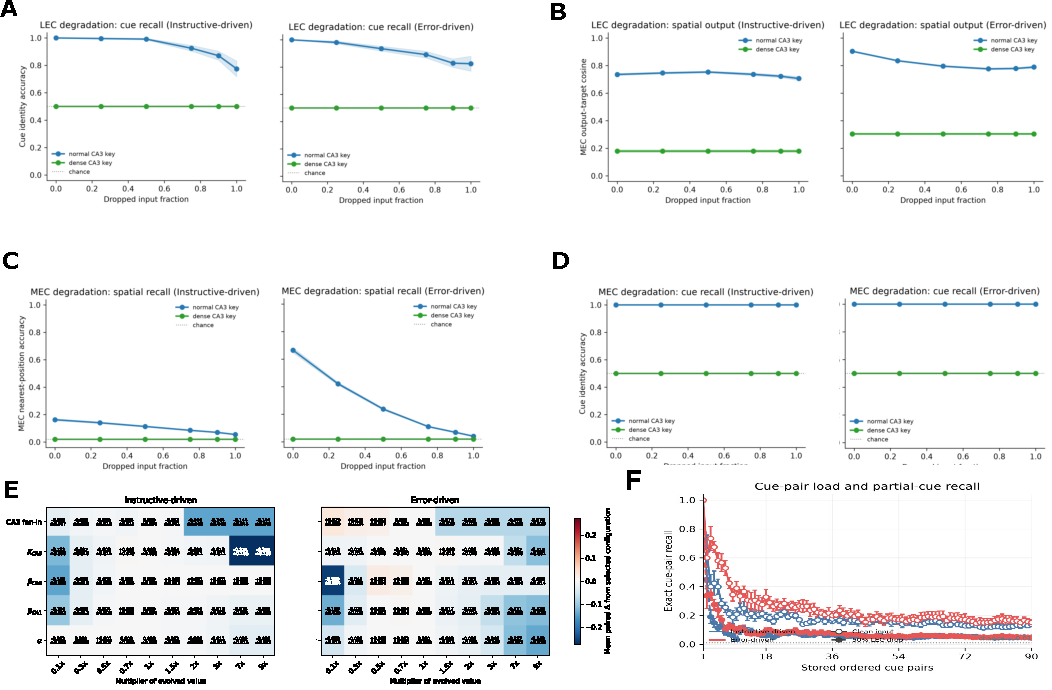
\includegraphics[width=\textwidth]{figure_3.pdf}
    \caption{\textbf{Selective degradation, parameter sensitivity, and
    cue-pair load.} In panels A--D, each pair of plots shows the
    instructive-driven rule on the left and the error-driven rule on the right.
    \textbf{(A)} Cue-identity accuracy during
    LEC-only degradation.
    \textbf{(B)} MEC output--target cosine during LEC-only degradation.
    \textbf{(C)} MEC nearest-position accuracy during MEC-only degradation.
    \textbf{(D)} Cue-identity accuracy during MEC-only degradation. Curves show
    mean $\pm$ SEM across 20 seeds after averaging 12 masks within each seed.
    Blue denotes the normal sparse CA3-like retrieval map; green denotes the
    dense common-key control, which collapses item-specific key structure and
    is not sparsity matched. Dotted horizontal lines denote chance accuracy
    where applicable. All degraded probes were performed with plasticity
    disabled. \textbf{(E)} Change in the three-component composite recall
    score when one MTL parameter was multiplied by the indicated factor while
    all others were held at that rule's evolved value. Integer parameters were
    rounded and model-valid bounds were enforced; each cell shows the paired
    mean score change over 10 independent seeds and its across-seed standard
    deviation. \textbf{(F)} Exact recall of
    ordered cue pairs as the number stored increased from 1 to 90. Blue denotes
    the instructive-driven rule and red the error-driven rule; open solid curves use intact probes and filled dashed
    curves use 50\% LEC dropout. Points show mean $\pm$ SEM across 10 held-out
    seeds, and the dotted line marks chance ($1/100$). Panels E and F use
    separately evolved rule-specific configurations and therefore compare
    operating regimes, whereas panels A--D use the shared reference
    configuration to isolate the update rule.}
    \label{fig:degradation}
\end{figure}

\FloatBarrier

\section{Discussion}

The central result is a representational constraint rather than a new claim
about hippocampal capacity. In this minimal architecture, a CA3-like retrieval
key selects associative content, plastic CA3--CA1 weights express that content
as a CA1 state, and a fixed decoder determines whether the state remains usable
at the output. A coordinate permutation preserves the instructed vector's
values yet disrupts reconstruction when the decoder is not transformed with
it. The matched-decoder rescue makes the logic exact: rapid plasticity must
preserve, or co-adapt with, the representational coordinates assumed by
recipient circuits. This motivates viewing CA1 not only as a locus of
experience-dependent activity, but also as an adaptive interface that places
retrieved content within a structured neural space. Such a space could allow
successive experiences to remain decodable even while individual fields and
participating neurons change.

This proposal complements rather than replaces existing accounts of
hippocampal memory. Autoassociative CA3 theories explain how a stored state can
be selected from a partial cue, whereas BTSP models explain how temporally broad
instructive events can rapidly alter CA1 synapses
\citep{nakazawa2002,bittner2017,wu2025}. The present model abstracts selection
as a non-recurrent CA3-like key and asks what must additionally hold when the
selected state is expressed at hippocampal output. The relationship to
neural-manifold work is conceptual: those studies concern motor cortical
learning, not hippocampal memory, but similarly show that an unchanged readout
assigns meaning only to particular population coordinates
\citep{sadtler2014,golub2018}. Readout compatibility is therefore a general
systems constraint instantiated here in a hippocampal circuit motif. The
simulations do not test retention across days or years; long-term decodability
is a hypothesis about what preserving this relation might enable, not an
observed outcome.

Pretraining and rapid plasticity have distinct computational roles in this
proposal. Pretraining establishes a sparse representational basis together with
the decoder that gives its coordinates meaning; rapid CA3--CA1 learning then
places a new, key-addressable experience within that basis. This resembles
feature reuse after pretraining in deep networks \citep{yosinski2014}, but the
analogy is functional rather than mechanistic. Likewise, the covariance matrix
adaptation evolution strategy (CMA-ES) used during preliminary model
development was an engineering procedure for locating a workable parameter
regime, not a proposed neural learning mechanism. In a biological circuit, the
basis could reflect development, prior learning, and ongoing
entorhinal--hippocampal organization rather than a separate optimization phase.
The frozen decoder is an assay of compatibility, not a claim that biological
recipient pathways are immutable. The broader prediction is that changes in a
CA1 code and its downstream readouts must remain coordinated.

The cue-track simulations connect readout compatibility to context-dependent
reconfiguration. Exchanging cue identities produced abrupt changes in recalled
CA1 tuning under both plasticity rules, whereas matched no-swap controls
remained stable at the same lap boundaries. Event alignment showed that most
of the change occurred on the first exchanged-cue lap and that consecutive-lap
similarity largely recovered on the next lap. Population-map similarity formed
alternating blocks: representations were similar within a cue assignment and
again when that assignment recurred, rather than drifting monotonically across
the experiment. After learning, both rules produced continuous mixtures of
spatially stable and cue-modulated units, with broad unit-level endpoint
similarities. This behavior is qualitatively consistent with cue-sensitive
field and rate changes and with evidence that EC-directed BTSP can form, shift,
and stabilize CA1 fields around behaviorally relevant features
\citep{leutgeb2005,grienberger2022,madar2025,vaidya2025}. On this
interpretation, instructed plasticity acts as an update operation on a spatial
cognitive map: it can insert, weaken, or reposition fields as relevant cues
change. In the present two-context task, the block structure is better
described as cue-dependent re-expression and updating than as the formation of
an unconstrained new map at every transition. The simulations are not a
quantitative model of biological remapping, however, and the unit distributions
were not compared with recorded field statistics. Their narrower implication
is that reconfiguration should be evaluated not only by how much CA1 activity
changes, but also by whether the new population state remains interpretable at
the output.

Comparing the two update rules clarifies why the form of rapid plasticity
matters. The instructive-driven rule produced stronger one-shot reconstruction and a larger
drop in tuning similarity at cue exchanges, followed by a more gradual recovery
over the next laps. The error-driven rule performed a bounded residual
correction and recovered most consecutive-lap stability by the following lap;
after repeated track experience it also produced greater spatial stability and
much higher clean position accuracy. These
differences should not be reduced to a single ranking. The instructive-driven
rule is closer in spirit to an instructed write, whereas the error-driven rule
adds a computational mechanism
for correcting under- and overexpressed CA1 components. Because both rules used
one shared parameter regime, their comparison reveals consequences of the
update signal under matched conditions rather than the best performance each
could achieve. A stronger model comparison would optimize each rule
independently and vary memory load, cue overlap, and learning rate.

The degradation experiments distinguish robustness to partial input from
mechanistic pattern completion. With the normal key map, recall remained
informative after substantial input loss, and selective removal of MEC-like or
LEC-like activity preferentially affected the corresponding readout. Yet the
CA3-like population has no recurrent connections or attractor settling.
Robustness arises from a distributed feedforward input-to-key map followed by a
learned key-to-content association. Degraded-cue recall alone therefore does
not identify a recurrent completion mechanism. A biological claim about CA3
pattern completion would require explicit recurrent dynamics and comparison
with interventions that alter those dynamics \citep{nakazawa2002,li2024}.

The dense common-key control also has a deliberately narrow interpretation. It
forces all CA3-like units to receive the same EC average and thus destroys
item-specific key structure while changing connection density and sparsity. Its
failure shows that a non-specific common key cannot support these associations;
it does not show that the selected sparse wiring is uniquely necessary or
optimal. Likewise, the MEC/LEC dissociation is partly expected from the
constructed input and readout partitions. Its value is as an internal
validation that the shared CA1 basis can retain access to an intact component,
not as evidence for strict anatomical modularity. Sparsity-matched controls
would be needed to separate the effects of connection density, dimensionality,
and key discriminability.

Several additional limitations define the scope of the work. The model omits
dentate gyrus, recurrent CA3 dynamics, attractor competition, inhibition,
consolidation, and explicit long-term drift of neurons or readouts. MEC and LEC
are simplified input halves despite mixed selectivity in both regions. The CA1
basis is obtained from a shallow autoencoder rather than a biologically
specified developmental process, and the plasticity equations are bounded
abstractions rather than temporal or molecular models of BTSP. The
compatibility manipulation is deliberately synthetic, and its matched-decoder
rescue is an equivariance control rather than independent biological evidence.
Finally, the track contains only two cue identities at one memory load;
capacity, interference, and scaling across multiple cue-pair sequences remain
unresolved.

These limitations suggest direct next tests. Model performance should depend
more strongly on compatibility between an instructed CA1 state and its output
basis than on the magnitude of CA1 change alone. Degraded-cue recall should
track retrieval-key discriminability across sparsity-matched controls, and
increasing the number of cue-pair sequences should eventually reveal an
interference-dependent capacity limit. Experimentally, the broad prediction is
that learning-related CA1 reconfiguration can remain behaviorally useful when
recipient populations preserve or acquire an appropriate readout, whereas an
equally large but readout-incompatible change should impair retrieval.

Within these bounds, the model offers a compact proposal linking a previously
established representational basis, rapid instructed plasticity,
retrieval-key-based selection, and downstream readability. CA1 activity can
change as a cognitive map is updated yet remain useful if retrieved content is
expressed in coordinates that recipient circuits can interpret. Readout
compatibility is therefore a useful axis for evaluating models of rapid
hippocampal learning and for asking how a changing hippocampal code might
support decodable experience over longer timescales.

\section{Methods}

\subsection{Implementation, reproducibility, and statistical treatment}

Simulations were implemented in Python using NumPy and PyTorch and run on CPU.
All reported experiments used the same 20 root seeds (51001--51020).
Conditions and plasticity rules within an experiment were paired by root seed.
The experiment scripts write a resolved JSON configuration, compressed NumPy
arrays, and a tidy CSV source-data table; plotting functions generate the
individual panels from those saved arrays. The composed vector figures do not
alter the underlying values.

During preliminary development, bounded hyperparameter configurations were
explored using the covariance matrix adaptation evolution strategy (CMA-ES).
This outer-loop engineering search used reconstruction- or recall-based
objectives to locate workable regimes for population sparsity, activation gain,
EC--CA3 convergence, and plasticity rate. The reported configurations were then
fixed before the 20-seed comparisons. CMA-ES was not applied separately to
individual seeds, experimental conditions, or plasticity rules; it is distinct
from both Adam-based autoencoder pretraining and the local CA3--CA1 updates
studied here.
In generic form, the search proposed bounded parameter vectors $\theta$ and
maximized a development-set score
\begin{equation}
J(\theta)=\frac{1}{N_{\mathrm{dev}}}
 \sum_{n=1}^{N_{\mathrm{dev}}}
 \operatorname{cos}\!\left(
 \widehat x_{\mathrm{EC}}^{(n)}(\theta),x_{\mathrm{EC}}^{(n)}\right),
\end{equation}
or its reconstruction-loss analogue. This procedure selected a computational
operating point; it was not included as evidence for learning, remapping, or
robustness, and optimization generations were not counted as experimental
replicates.

The unit of computational replication was the root seed, not an individual
memory, CA1 unit, track position, or corruption mask. Values were first
averaged over observations nested within a seed and then summarized across
seeds. For a seed-level statistic $y_s$, $s=1,\ldots,S$, curves and error bars
show $\bar y\pm\operatorname{SEM}(y)$, where
\begin{equation}
\bar y=\frac{1}{S}\sum_{s=1}^{S}y_s,\qquad
\operatorname{SEM}(y)=
\sqrt{\frac{1}{S(S-1)}\sum_{s=1}^{S}(y_s-\bar y)^2}.
\end{equation}
Confidence intervals (CIs)
reported in the text are two-sided 95\% Student-$t$ intervals over the 20
seed-level values,
$\bar y\pm t_{0.975,S-1}\operatorname{SEM}(y)$. Contrasts use paired
seed-level differences $d_s=y_s^{(A)}-y_s^{(B)}$ rather than differences
between independently aggregated conditions. These intervals
quantify sensitivity to sampled initializations and inputs, not uncertainty
over a biological population. No null-hypothesis significance tests or
multiple-comparison corrections were applied; all analyses are descriptive
simulation results.

\subsection{EC patterns and the pretrained CA1 basis}

EC input, CA1, and CA3-like populations each contained 50 units. A one-hidden-
layer autoencoder mapped EC input to a 50-unit CA1 representation and back to a
50-unit EC output. CA1 activity used a differentiable top-$K$ sparse activation
with $K_{\mathrm{CA1}}=5$ and inverse temperature $\beta=25$; output activity
used a sigmoid decoder with gain 25. Linear encoder and decoder biases were
disabled. Specifically, if $z_{(1)}\geq\cdots\geq z_{(N)}$ are the sorted
preactivations, the activation threshold and sparse nonlinearity were
\begin{align}
\vartheta_K(z) &= \frac{z_{(K)}+z_{(K+1)}}{2},\\
[\mathcal{S}_{K,\beta}(z)]_i
 &= \sigma\!\left(\beta[z_i-\vartheta_K(z)]\right),
\qquad \sigma(u)=\frac{1}{1+e^{-u}}.
\label{eq:sparse-activation}
\end{align}
Thus approximately $K$ units lay above the adaptive half-activation threshold,
while gradients remained defined near that threshold. For EC pattern
$x_{\mathrm{EC}}\in\{0,1\}^{50}$, encoder $E$, and decoder $D$, pretraining
computed
\begin{align}
x_{\mathrm{IS}} &= \mathcal{S}_{5,25}(E x_{\mathrm{EC}}),\\
\widetilde{x}_{\mathrm{EC}} &= \sigma(25D x_{\mathrm{IS}}),\\
\mathcal{L}_{\mathrm{AE}} &=
 \frac{1}{N}\sum_{n=1}^{N}
 \left\|\widetilde{x}_{\mathrm{EC}}^{(n)}
             -x_{\mathrm{EC}}^{(n)}\right\|_2^2.
\label{eq:autoencoder}
\end{align}
The weights were trained with Adam (learning rate 0.001, batch size 64) to
minimize Eq.~\ref{eq:autoencoder}. Pretraining occurred before
CA3--CA1 storage, after which the encoder and decoder were fixed. The encoder
therefore supplied the instructed CA1 state (IS), and the decoder defined the
output coordinates against which compatibility was tested.

For the readout-compatibility experiment, the autoencoder was trained for 1024
epochs on 2048 unique binary EC patterns with five active units and evaluated
on 256 held-out patterns. Twenty-eight additional unique patterns were reserved
for one-shot associative storage. For the cue-reconfiguration experiment, the
autoencoder was trained for 256 epochs on the 40 training laps and evaluated on
10 separately generated laps. For the degradation experiment, it was trained
for 256 epochs on 20 intact laps and evaluated on five separately generated
laps. Each lap contained 50 positions.

Track inputs contained 25 MEC-like and 25 LEC-like units. For position
$p\in\{0,\ldots,L-1\}$ on a circular track of length $L=50$, circular distance
was $d_L(p,\mu)=\min(|p-\mu|,L-|p-\mu|)$. MEC unit $i$ had a preferred position
$\mu_i$ from an even tiling of the track and Gaussian activation probability
\begin{equation}
g_i(p)=\exp\!\left[-\frac{1}{2}
 \left(\frac{d_L(p,\mu_i)}{\sigma_{\mathrm{MEC}}}\right)^2\right],
\qquad \sigma_{\mathrm{MEC}}=5.
\end{equation}
Binary MEC activity was sampled independently as
$x_{\mathrm{MEC},i}(p)\sim\operatorname{Bernoulli}(g_i(p))$. Two fixed,
non-overlapping 25-dimensional LEC cue templates $q_1$ and $q_2$ were centered
at $c_1=10$ and $c_2=30$. Cue $j$ was present with probability
\begin{align}
g_j^{\mathrm{cue}}(p)
 &=\exp\!\left[-\frac{1}{2}
 \left(\frac{d_L(p,c_j)}{4}\right)^2\right],\\
P_j(p)&=\operatorname{clip}_{[0,1]}
 \left\{2\sigma\!\left(40[g_j^{\mathrm{cue}}(p)-0.1]\right)-1\right\}.
\end{align}
If the Bernoulli cue-presence sample was positive, the LEC block was set to
$q_j$; otherwise it was zero. The complete entorhinal target was the
concatenation $x_{\mathrm{EC}}(p)=[x_{\mathrm{MEC}}(p);
x_{\mathrm{LEC}}(p)]$. This stochastic construction generated different laps
from the same underlying spatial and cue statistics.

\subsection{CA3-like retrieval keys and CA3--CA1 plasticity}

EC input was projected to 50 CA3-like units through a fixed sparse matrix
followed by a differentiable top-$K$ activation. The compatibility experiment
used two EC inputs per CA3-like unit, $K_{\mathrm{CA3}}=5$, inverse-temperature
parameter $\beta_{\mathrm{CA3}}=200$, and learning rate $\alpha=0.08$. Track
experiments used 29 EC inputs per CA3-like unit, $K_{\mathrm{CA3}}=3$,
$\beta_{\mathrm{CA3}}=170.6$, and $\alpha=0.092$. The normal track map was
constructed to balance EC participation across CA3-like units.
CA3--CA1 weights were initialized to zero. The CA1 recall activation used
$K_{\mathrm{CA1}}=5$, with inverse temperature 25 in the compatibility
experiment and 41.8 in the track experiments.

Writing and recall used the same fixed EC--CA3 projection $A$ and frozen
decoder $D$. At weight state $W_t$, the complete forward computation was
\begin{align}
x_{\mathrm{CA3}} &=
 \mathcal{S}_{K_{\mathrm{CA3}},\beta_{\mathrm{CA3}}}
 (A x_{\mathrm{EC}}),\\
x_{\mathrm{CA1}} &=
 \mathcal{S}_{5,\beta_{\mathrm{CA1}}}(W_t x_{\mathrm{CA3}}),\\
\widehat{x}_{\mathrm{EC}} &= \sigma(25D x_{\mathrm{CA1}}).
\label{eq:recall-forward}
\end{align}
Each selected input to a CA3-like unit had projection weight $1/50$; all other
entries of $A$ were zero. Consequently, the convergence parameter controlled
which EC components contributed to a key, whereas the top-$K$ nonlinearity
controlled key population sparsity. Equation~\ref{eq:recall-forward} was also
used to compute the pre-update recall state required by the error-driven rule.

Let $x_{\mathrm{EC}}$ denote the EC input/target,
$x_{\mathrm{CA3}}$ its retrieval key, $x_{\mathrm{IS}}$ the instructed CA1
state produced by the fixed encoder, and $x_{\mathrm{CA1}}$ the state recalled
through the current CA3--CA1 weights $W_t$. The instructive-driven update was
\begin{equation}
W_{t+1} =
  (1-\alpha x_{\mathrm{IS}})\odot W_t
  + \alpha x_{\mathrm{IS}}x_{\mathrm{CA3}}^{\mathsf T},
\label{eq:instructive-driven-rule}
\end{equation}
where the first term is broadcast across presynaptic dimensions. For the
bounded error-driven rule,
\begin{align}
e^+ &= [x_{\mathrm{IS}}-x_{\mathrm{CA1}}]_+, &
e^- &= [x_{\mathrm{CA1}}-x_{\mathrm{IS}}]_+,\\
\delta^+ &= \alpha(e^+x_{\mathrm{CA3}}^{\mathsf T})(1-W_t), &
\delta^- &= \alpha(e^-x_{\mathrm{CA3}}^{\mathsf T})W_t,\\
W_{t+1} &= \operatorname{clip}_{[0,1]}
           (W_t+\delta^+-\delta^-).
\label{eq:error-driven-rule}
\end{align}
Recalled CA1 activity was obtained by applying the same target sparsity to
$W_tx_{\mathrm{CA3}}$ and was passed through the fixed pretrained decoder.
The instructive-driven rule depends on the instructed target and presynaptic key but not
the current recall error. The error-driven rule separates the residual into
positive and negative components, such that under- and overexpressed CA1
components drive bounded potentiation and depression, respectively.
All products between equally shaped arrays were elementwise unless an outer
product or matrix product is shown explicitly. Memories were presented
sequentially, and $W_{t+1}$ was carried to the next item or position without
replay, batching, or gradient descent through the local plasticity dynamics.

\subsection{Paired plasticity-rule design}

Both rules were evaluated in every main experiment. Within a root seed they
shared EC inputs, pretrained autoencoder weights, CA3 wiring seeds, storage
order, and--in the degradation experiment--corruption masks. Each rule had its
own CA3--CA1 weight matrix, which evolved according to the corresponding
update. All memory hyperparameters were shared rather than optimized for each
rule. Supplementary Fig.~\ref{fig:rule-comparison} collects four paired contrasts
derived directly from the main result arrays; it is not a separate simulation.

\subsection{Readout-compatibility experiment}

For each seed, the 28 held-out EC patterns were assigned CA3-like retrieval keys
and pretrained CA1 instructions, then written once in a shared random order.
The aligned condition used the original IS and decoder. The fixed-permutation
condition applied one seed-specific CA1 permutation to every IS while leaving
the decoder unchanged. The matched-decoder condition used the same permuted
instructions and correspondingly permuted decoder columns. The random-content
condition associated each key with a shuffled memory instruction. The
no-plasticity condition retained zero CA3--CA1 weights. Recall was evaluated
using cosine similarity between reconstructed EC output and the corresponding
EC target. Each seed's plotted value is its mean across 28 memories.

More explicitly, let $P$ be the permutation matrix and $h=x_{\mathrm{IS}}$.
The aligned condition stored $h$ and read it with $D$; the fixed-permutation
condition stored $Ph$ but retained $D$; and the matched-decoder condition used
$Ph$ together with $D'=DP^{\mathsf T}$. In the idealized exact-recall case,
\begin{equation}
D'Ph=DP^{\mathsf T}Ph=Dh,
\end{equation}
so matched decoder relabeling restores the original output coordinates without
restoring the original CA1 unit identities. This control isolates coordinate
compatibility from a generic effect of permutation. Similarity between two
nonzero vectors $u$ and $v$ was
\begin{equation}
\operatorname{cos}(u,v)=\frac{u^{\mathsf T}v}
 {\lVert u\rVert_2\lVert v\rVert_2};
\end{equation}
zero-norm cases were assigned similarity zero by the numerical implementation.

\subsection{Cue-reconfiguration experiment}

Models learned 40 complete laps. Cue identities exchanged positions every 10
laps, alternating between assignments $[0,1]$ and $[1,0]$. The matched
no-swap schedule retained $[0,1]$ for all 40 laps. Within a seed, the schedules
shared the pretrained autoencoder, initial CA3--CA1 weights, MEC-like
trajectory, lap count, plasticity parameters, and the exact EC--CA3 projection;
only cue identity after the first 10 laps differed by design. Both plasticity
rules used this same projection. Thus all schedule contrasts in
Fig.~\ref{fig:compatibility}B,E,F are paired at the level of the root seed and
fixed retrieval-key wiring.

After each training lap, plasticity was paused while both fixed cue contexts
were probed; the probe matching the context scheduled for that lap was retained
for the transition analysis. For each CA1 unit, activity was mean-centered
across positions before calculating cosine similarity between consecutive
spatial tuning curves. Similarities were then averaged across units. Cue-exchange
transitions were compared with the same lap boundaries in the paired no-swap
model.

Let $f_{\ell c i}(p)$ be the frozen-probe activity of CA1 unit $i$ at position
$p$, after training lap $\ell$, under cue context $c$, and define the centered
curve $\widetilde f_{\ell c i}(p)=f_{\ell c i}(p)-L^{-1}
\sum_{r=0}^{L-1}f_{\ell c i}(r)$. Consecutive-lap tuning similarity was
\begin{equation}
T_\ell=\frac{1}{N_{\mathrm{CA1}}}\sum_{i=1}^{N_{\mathrm{CA1}}}
 \operatorname{cos}(\widetilde f_{\ell c_\ell i},
                    \widetilde f_{\ell-1,c_{\ell-1},i}).
\label{eq:transition-similarity}
\end{equation}
The transition statistic compared $T_\ell$ at boundaries
$\ell\in\{10,20,30\}$ with the same boundaries in the matched no-swap run.

For the exact-wiring event analysis, each boundary $e\in\{10,20,30\}$ was
treated as relative lap $\tau=0$, the first lap learned under the exchanged
cue assignment. The analysis window was $\tau\in\{-3,\ldots,9\}$. Let
$c_{e+\tau}$ be the context scheduled at that relative lap. The final
pre-exchange probe and the final probe of the ensuing ten-lap block defined
the old and adapted references, respectively:
\begin{align}
R_{\mathrm{old}}(e,\tau)
 &=\frac{1}{N_{\mathrm{CA1}}}\sum_i
 \operatorname{cos}\!\left(
 \widetilde f_{e+\tau,c_{e+\tau},i},
 \widetilde f_{e-1,c_{e-1},i}\right),\\
R_{\mathrm{adapt}}(e,\tau)
 &=\frac{1}{N_{\mathrm{CA1}}}\sum_i
 \operatorname{cos}\!\left(
 \widetilde f_{e+\tau,c_{e+\tau},i},
 \widetilde f_{e+9,c_{e+9},i}\right).
\label{eq:remapping-references}
\end{align}
The adapted reference is retrospective: it describes convergence toward the
state reached at the end of a block and is not a prediction of a future map.
Consecutive-lap similarity used Eq.~\ref{eq:transition-similarity} at each
$e+\tau$. Values were first averaged over the three events within a root seed
and then summarized across seeds. The no-swap control was indexed by the same
nominal boundaries, although its cue assignment did not change.

For the population representational-similarity matrix, the complete
position-by-unit probe map after lap $\ell$ was centered independently for each
unit over position and vectorized as
\begin{equation}
v_\ell=\operatorname{vec}\!\left[
f_\ell-\frac{1}{L}\mathbf{1}\mathbf{1}^{\mathsf T}f_\ell
\right],\qquad
P_{\ell m}=\operatorname{cos}(v_\ell,v_m).
\label{eq:population-map-similarity}
\end{equation}
The displayed matrix is the elementwise mean of $P$ across 20 root seeds.
Unit-level endpoint similarity was
$U_{ei}=\operatorname{cos}(\widetilde f_{e-1,c_{e-1},i},
\widetilde f_{e+9,c_{e+9},i})$. Its empirical cumulative distribution was
computed within each seed after pooling that seed's three exchange events;
the plotted curve and uncertainty were then calculated across seeds, avoiding
treatment of individual CA1 units as independent replicates.

After the final lap, plasticity remained frozen and the two cue contexts were
probed. For each CA1 unit, spatial stability was the cosine similarity between
its two mean-centered context tuning curves. Cue modulation was the mean
absolute activity difference between contexts. These metrics quantify context
sensitivity but do not themselves classify rate or global remapping. Heat maps
show the error-driven seed whose mean stability and modulation were closest to the
across-seed medians; units were ordered by preferred position across the two
contexts.
For final-lap contexts $a$ and $b$, the plotted unit-level quantities were
\begin{align}
S_i &= \operatorname{cos}(\widetilde f_{a i},\widetilde f_{b i}),\\
M_i &= \frac{1}{L}\sum_{p=0}^{L-1}|f_{a i}(p)-f_{b i}(p)|.
\end{align}
Here $S_i$ measures preservation of spatial profile after removing mean firing,
whereas $M_i$ retains absolute context-dependent rate differences; their joint
distribution therefore separates two complementary aspects of mixed tuning.

\subsection{Selective degradation experiments}

Models stored 20 intact laps with cue assignment $[0,1]$. During frozen recall,
a fixed random subset of eligible EC units was zeroed throughout a complete
probe lap. Masks were sampled independently between probes. Dropped fractions
were 0, 0.25, 0.50, 0.75, and 0.90, with 12 masks per fraction and root seed.
LEC-like degradation operated on the final 25 input units; MEC-like degradation
operated on the first 25.

For dropped fraction $q$ and mask replicate $r$, a binary mask
$m^{(q,r)}\in\{0,1\}^{50}$ set
$\operatorname{round}(25q)$ randomly selected coordinates in the targeted
input half to zero and left all other coordinates at one. The same mask was
held fixed for all positions of that probe lap:
\begin{equation}
x_{\mathrm{EC}}^{(q,r)}(p)=m^{(q,r)}\odot x_{\mathrm{EC}}(p).
\label{eq:degradation-mask}
\end{equation}
Plasticity was disabled during these probes, so degradation altered retrieval
evidence but did not rewrite the stored association.

Cue identity was decoded at the two cue positions by cosine comparison between
recalled LEC output and the two fixed cue templates. Spatial accuracy was the
fraction of recalled MEC outputs whose nearest clean MEC target had the correct
track-position index; chance was therefore $1/50$. MEC output cosine was
averaged across all positions. For every curve, the 12 mask-level values were
first averaged within a seed before means and uncertainty were calculated
across seeds.

Writing $\widehat x_{\mathrm{LEC}}(c_j)$ for recalled LEC output at cue center
$c_j$ and $x_{\mathrm{MEC}}^*(p)$ for the clean MEC target at position $p$,
the three reported metrics were
\begin{align}
A_{\mathrm{cue}}
 &=\frac{1}{2}\sum_{j=1}^{2}
 \mathbf{1}\!\left[j=\arg\max_{k\in\{1,2\}}
 \operatorname{cos}(\widehat x_{\mathrm{LEC}}(c_j),q_k)\right],\\
A_{\mathrm{pos}}
 &=\frac{1}{L}\sum_{p=0}^{L-1}
 \mathbf{1}\!\left[p=\arg\max_{u\in\{0,\ldots,L-1\}}
 \operatorname{cos}(\widehat x_{\mathrm{MEC}}(p),x_{\mathrm{MEC}}^*(u))\right],\\
C_{\mathrm{MEC}}
 &=\frac{1}{L}\sum_{p=0}^{L-1}
 \operatorname{cos}(\widehat x_{\mathrm{MEC}}(p),x_{\mathrm{MEC}}^*(p)).
\end{align}
Cue accuracy has two-class chance level $1/2$, whereas exact-position accuracy
has chance level $1/L=1/50$. MEC cosine is graded and has no corresponding
uniform-classification chance line.

The dense common-key control replaced the EC--CA3 map with a matrix whose every
entry was $1/50$. All CA3-like units consequently received the same average EC
input and generated a common, non-item-specific key. Because this control also
changes connection density and sparsity relative to the normal map, it tests
the need for key discriminability rather than the isolated effect of sparse
connectivity.
In matrix notation the control used $A_{ij}=1/50$ for all $i,j$; hence every
CA3 preactivation was identical for a given input. Equation~\ref{eq:sparse-activation}
therefore returned the same $0.5$-valued vector for every input, rather
than an item-specific key.


\section*{Data and code availability}

The simulations underlying Figs.~\ref{fig:compatibility},
\ref{fig:degradation}, and Supplementary Figs.~\ref{fig:rule-comparison} and
\ref{fig:remapping-dynamics} are generated by the scripts in
\texttt{src/experiments}. This includes the autoencoder and MTL CMA-ES
searches, local parameter-sensitivity analysis, and cue-pair load experiment.
Resolved configurations, selected parameter files, compressed numerical
arrays, and tidy source-data tables are stored in
\texttt{results/preprint}. A permanent public archive and accession identifier
will be added before public posting.

\begingroup
\small
\bibliographystyle{plainnat}
\bibliography{references}
\endgroup

\clearpage
\section*{Supplementary material}

\setcounter{figure}{0}
\renewcommand{\thefigure}{S\arabic{figure}}
\renewcommand{\theHfigure}{S\arabic{figure}}

\begin{figure}[H]
    \centering
    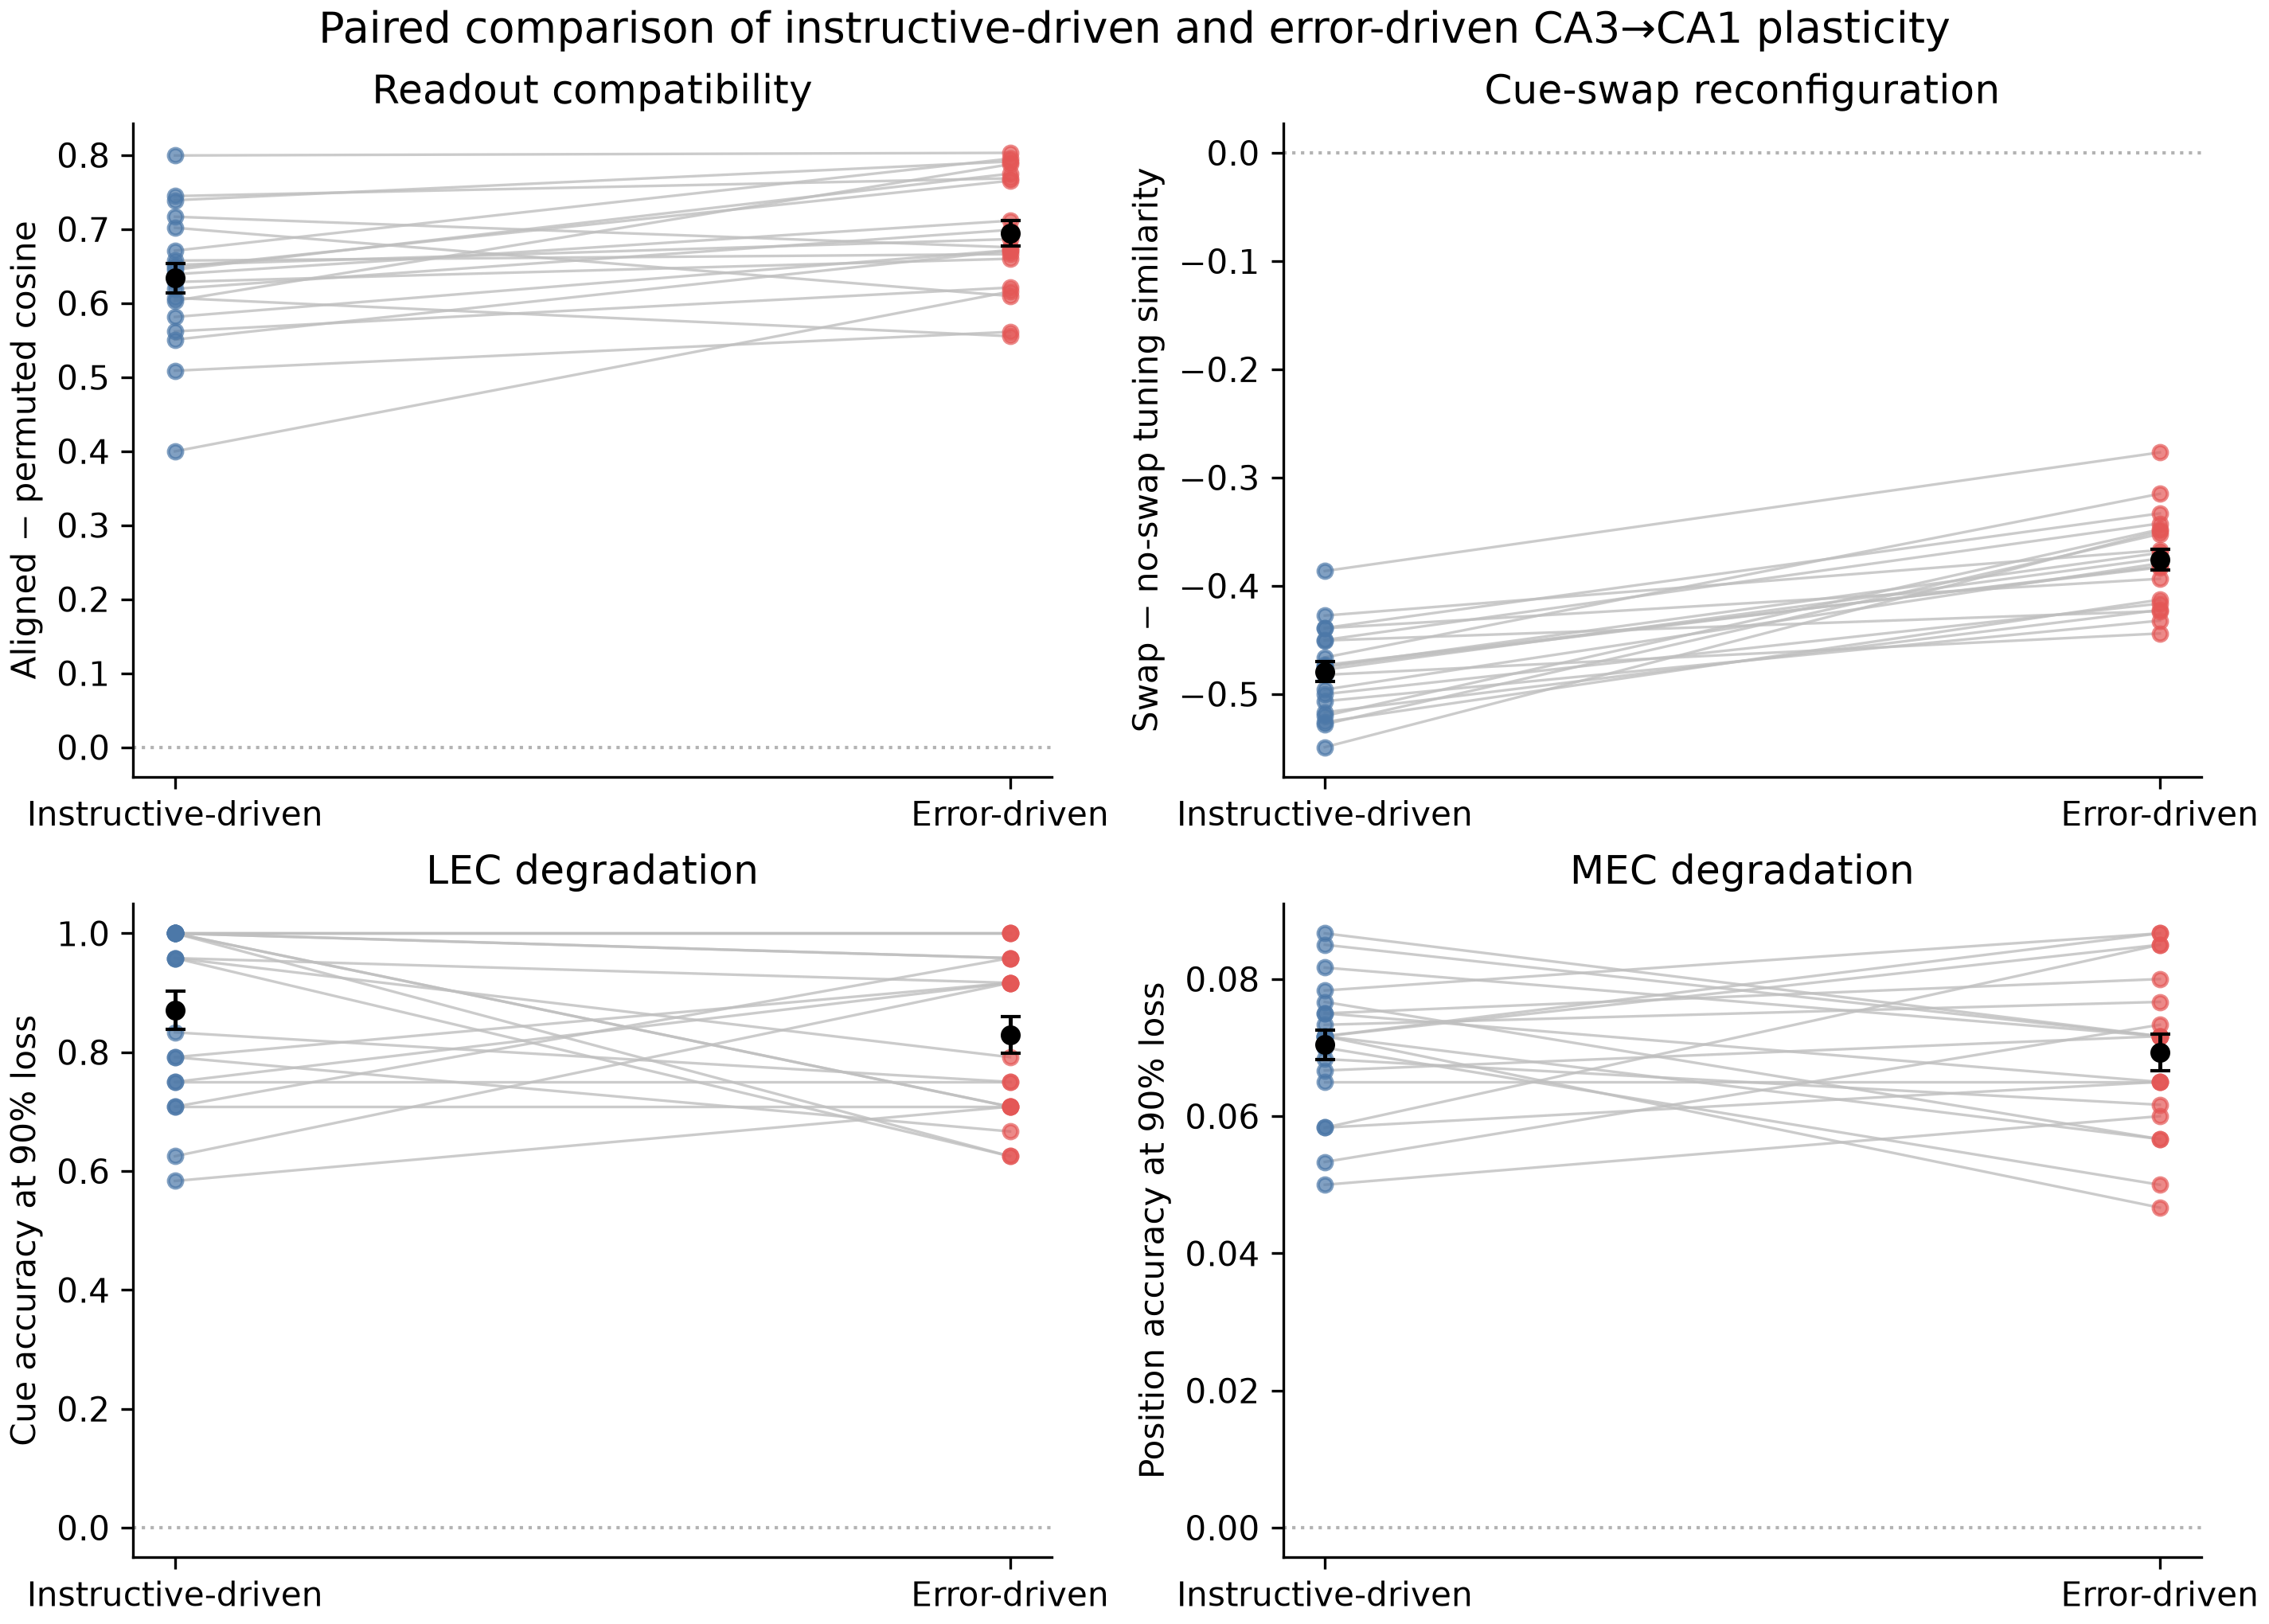
\includegraphics[width=\textwidth]{plasticity_comparison.png}
    \caption{\textbf{Seed-paired comparison of instructive-driven and
    error-driven plasticity.} Each grey line joins instructive-driven and
    error-driven values obtained from the
    same root seed; colored points are individual seed-level values and black
    points with error bars show mean $\pm$ SEM across 20 seeds.
    \textbf{(Upper left)} Readout-compatibility effect, defined as aligned minus
    fixed-permutation output--target cosine in Fig.~\ref{fig:compatibility}A.
    \textbf{(Upper right)} Cue-exchange effect, defined as tuning similarity at
    exchange boundaries minus similarity at the same boundaries in the
    no-swap control in Fig.~\ref{fig:compatibility}B.
    \textbf{(Lower left)} Cue identity accuracy after 90\% LEC-like degradation
    in Fig.~\ref{fig:degradation}A.
    \textbf{(Lower right)} Nearest-position accuracy after 90\% MEC-like
    degradation in Fig.~\ref{fig:degradation}C. Both rules shared inputs,
    pretrained autoencoders, CA3 wiring seeds, storage order, corruption masks,
    and hyperparameters; only
    the CA3--CA1 update differed. Parameters were not optimized separately for
    each rule.}
    \label{fig:rule-comparison}
\end{figure}

\begin{figure}[p]
    \centering
    \begin{minipage}[t]{0.48\textwidth}
    \textbf{A}\par
    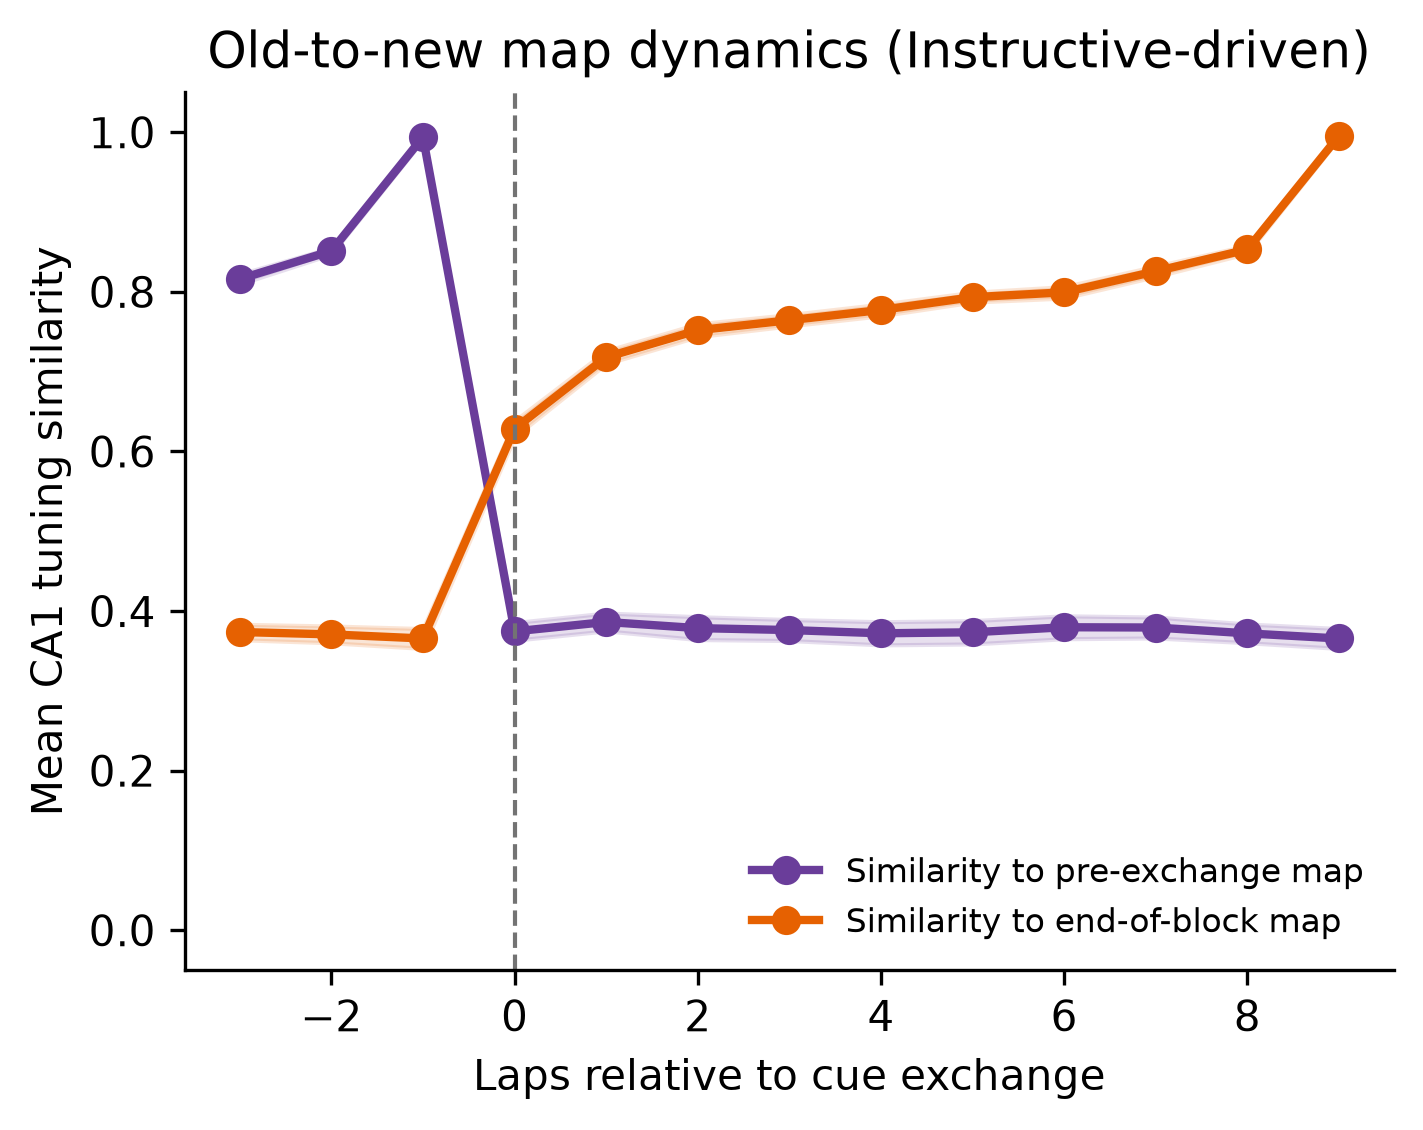
\includegraphics[width=\linewidth]{remapping_old_new_base.png}
    \end{minipage}
    \hfill
    \begin{minipage}[t]{0.48\textwidth}
    \textbf{B}\par
    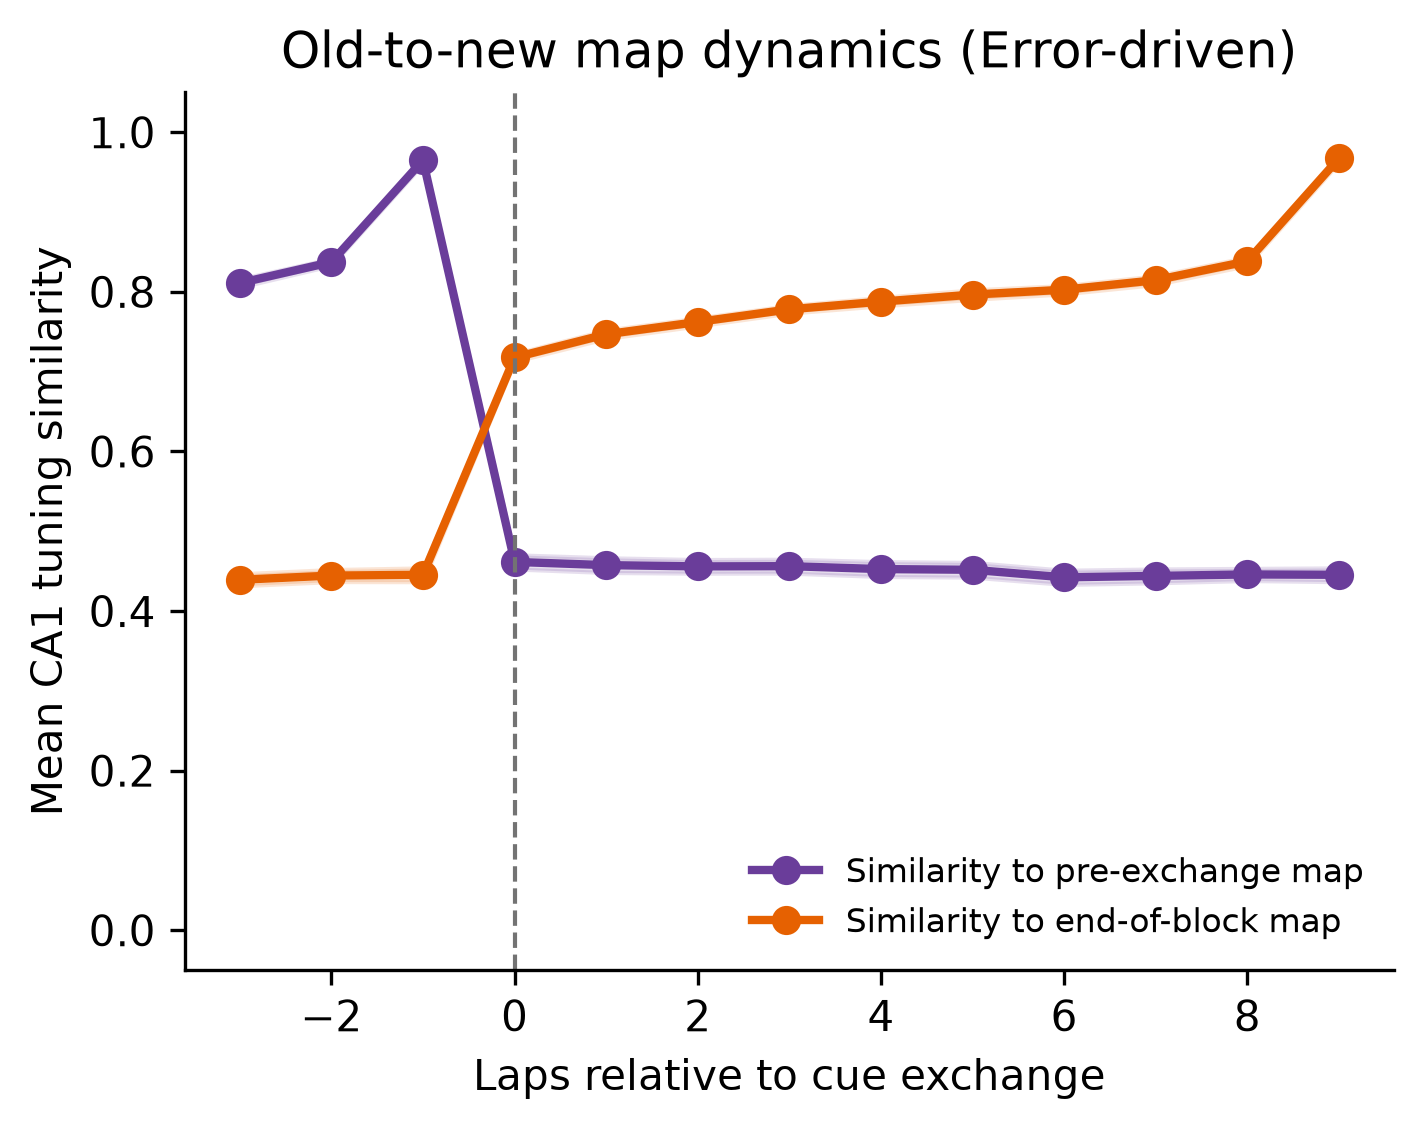
\includegraphics[width=\linewidth]{remapping_old_new_err2.png}
    \end{minipage}

    \vspace{0.5em}

    \begin{minipage}[t]{0.48\textwidth}
    \textbf{C}\par
    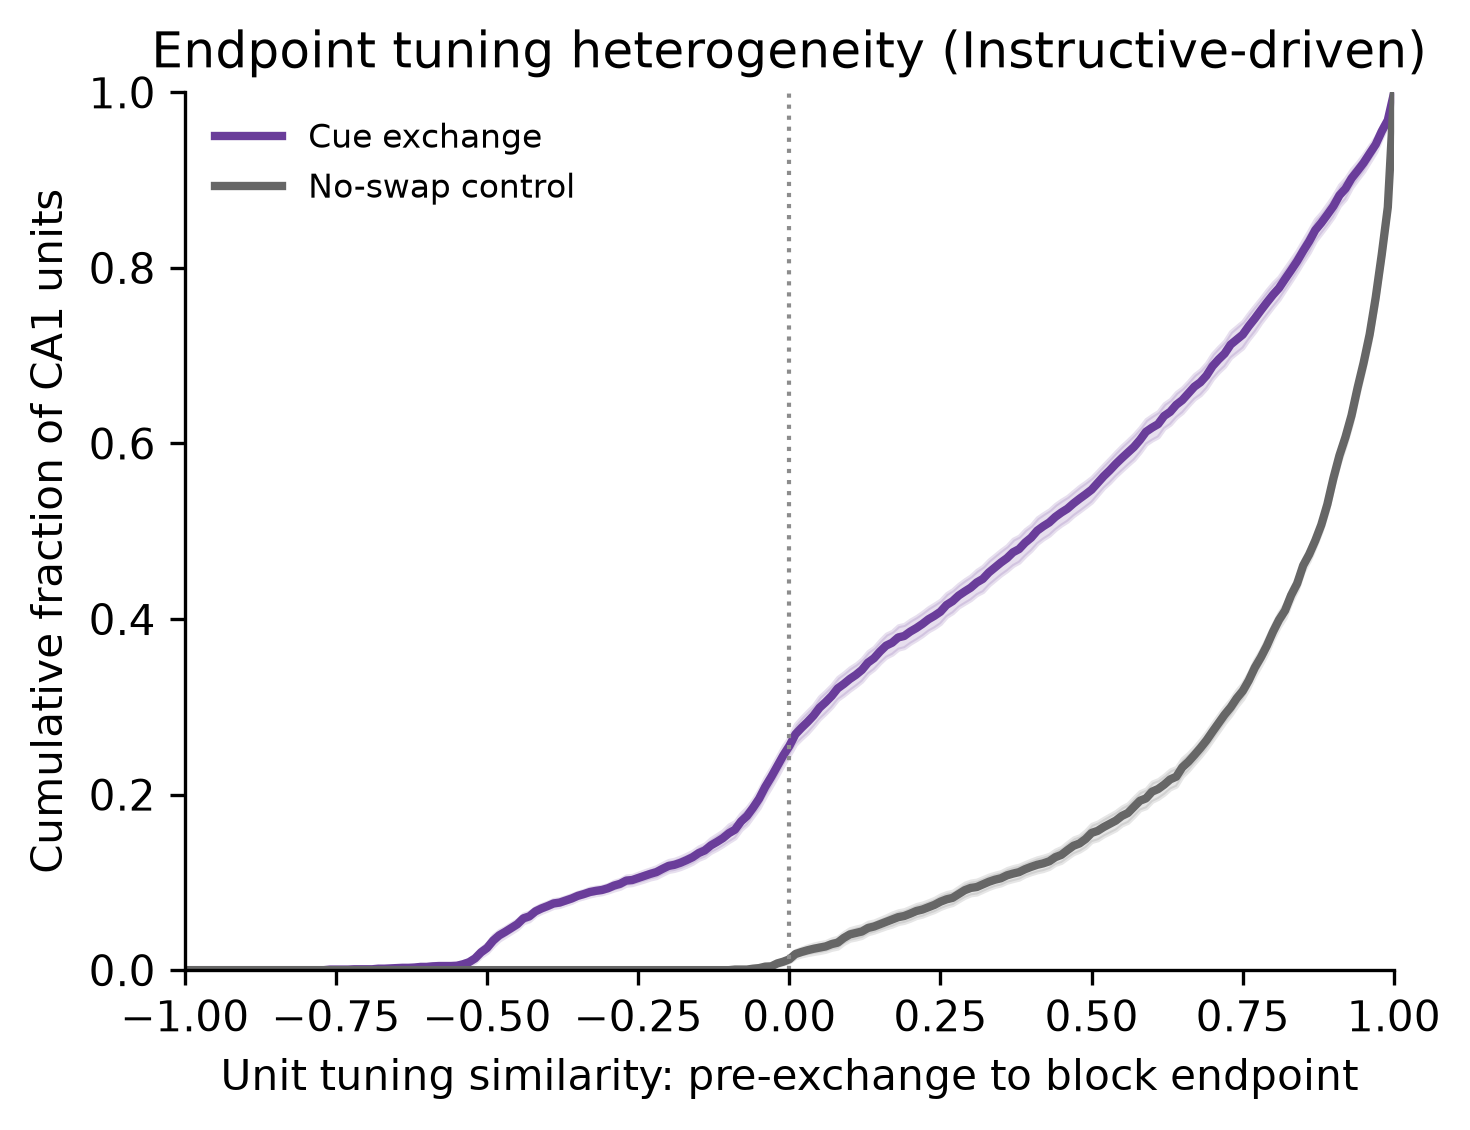
\includegraphics[width=\linewidth]{remapping_endpoint_base.png}
    \end{minipage}
    \hfill
    \begin{minipage}[t]{0.48\textwidth}
    \textbf{D}\par
    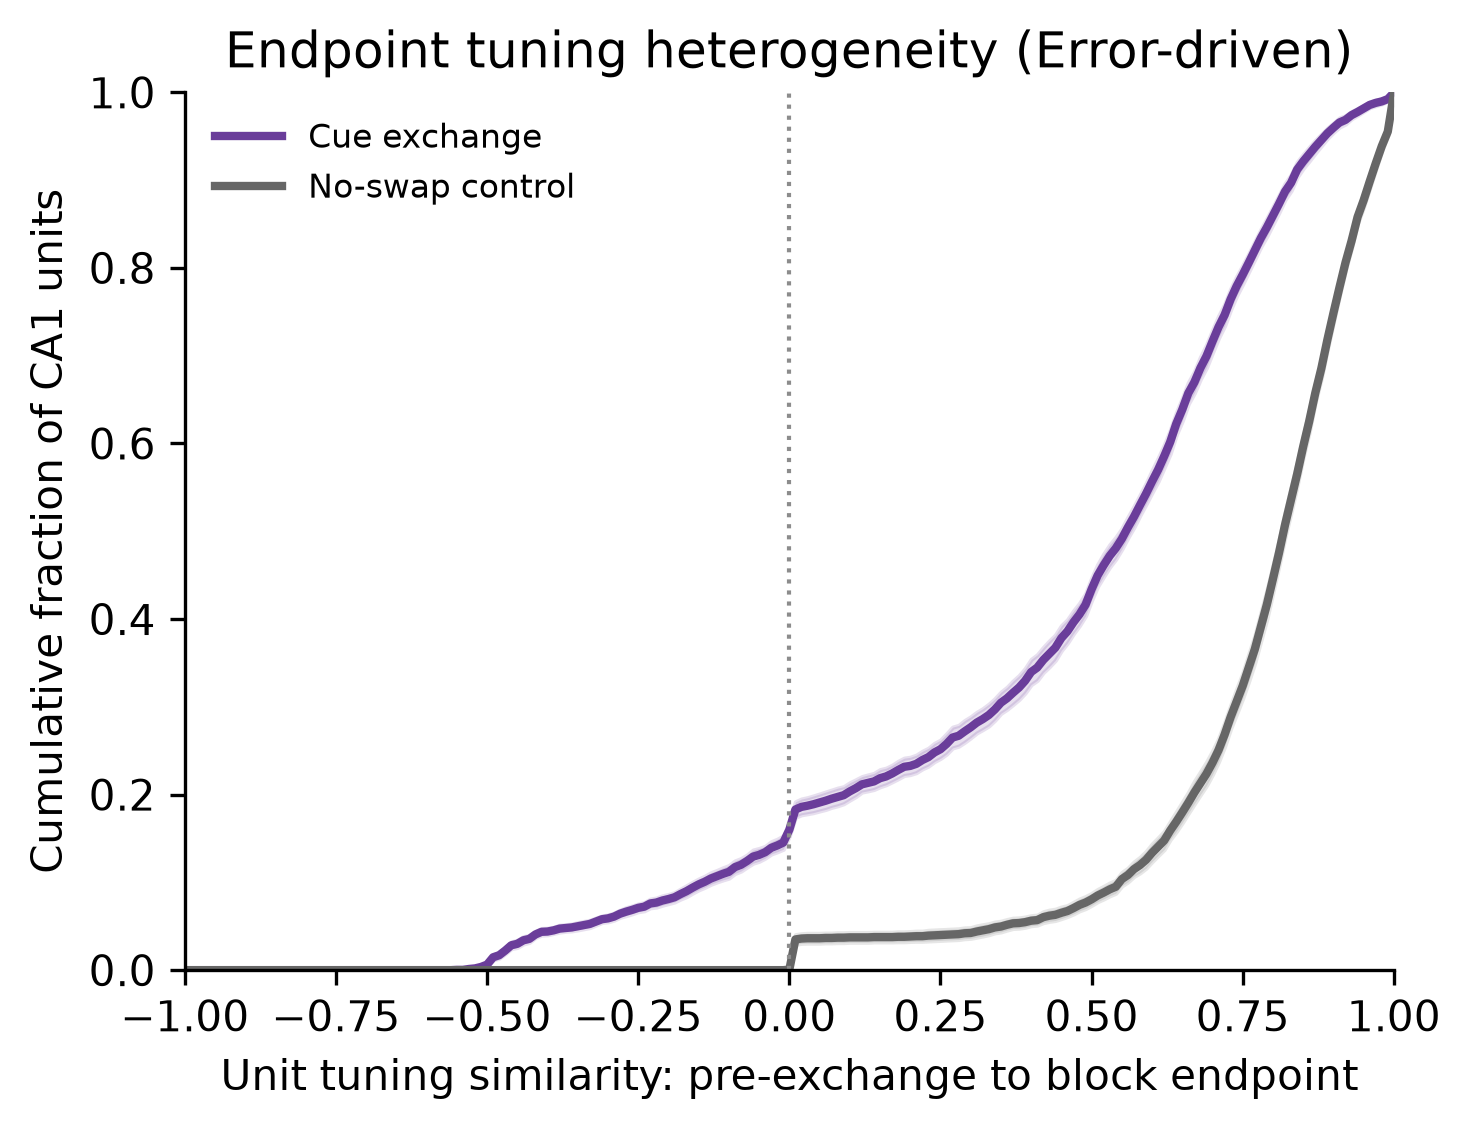
\includegraphics[width=\linewidth]{remapping_endpoint_err2.png}
    \end{minipage}
    \caption{\textbf{Reference-map dynamics and heterogeneity after cue
    exchange.} \textbf{(A,B)} Similarity of the current CA1 tuning map to the
    final pre-exchange map (purple) and to the final map of the ensuing
    ten-lap block (orange), for instructive-driven (A) and error-driven (B)
    plasticity. Relative lap zero is the first lap learned after cue exchange.
    The adapted-map reference is retrospective and therefore equals one at the
    block endpoint by construction; the informative result is the abrupt
    crossover at exchange followed by smaller within-block changes.
    \textbf{(C,D)} Seed-averaged empirical cumulative distributions of
    unit-level tuning similarity between the pre-exchange and block-end maps
    for instructive-driven (C) and error-driven (D) plasticity. Purple denotes
    cue exchange and grey the matched no-swap control. For every curve, events
    and units were aggregated within each root seed before the mean and SEM
    were calculated across 20 seeds. These distributions describe population
    heterogeneity and do not treat units as independent replicates. All panels
    use the exact same EC--CA3 projection in the exchange and no-swap
    schedules.}
    \label{fig:remapping-dynamics}
\end{figure}


\end{document}
